% Sample Paper for Poster Conference
%( without guarantee:-)) 
%send your comment to xrund@fel.cvut.cz
%
\documentclass{poster16}
% 
%----------------------------------------------------------
%             THIS IS THE PLACE FOR YOUR FAVORITE PACKAGES
%
%\usepackage[latin2]{inputenc}%
%\usepackage{babel}% 
%\usepackage{czech}%
%\usepackage{psfrag}
%\usepackage{amsmath}
%\usepackage{pifont,amssymb}

\begin{document}
%----------------------------------------------------------

%----------------------------------------------------------
%               THIS IS THE PLACE OF THE TITLE
%
\title{3D printed rocket - platform for student experiments}
%----------------------------------------------------------
%               THIS IS THE PLACE FOR THE AUTHORS NAMES AND THE TITLE FOR HEADINGS
%
\headtitle{F. S. AUTHOR, S. S. AUTHOR, SAMPLE PAPER FOR POSTER 2016 CONFERENCE}
%----------------------------------------------------------
%               THIS IS THE PLACE FOR THE AUTHORS NAMES - ALL AUTHORS MUST HAVE A STUDENT STATUS!!!

%
\author{Jakub Kakona \affiliationmark{1}}
%----------------------------------------------------------
%              THIS IS THE PLACE FOR AFFILIATIONS
%
\affiliation{%
\affiliationmark{1}Dept. of Radio engineering, Czech Technical University, Technick\'a 2, 166 27 Praha, Czech Republic}
  \email{kakonjak@fel.cvut.cz}
%--------------------------------------------------------------


\maketitle

%----------------------------------------------------------
%               THIS IS THE PLACE FOR ABSTRACT

\begin{abstract}
\end{abstract}


%----------------------------------------------------------
%               THIS IS THE PLACE FOR KEYWORDS
\begin{keywords}
Rocket experiments, 3D printing, sounding rocket, experimental platform.
\end{keywords}

%----------------------------------------------------------
%               HERE WRITE YOUR PAPER

\section{Introduction}

Scientific rocket experiments was relatively common in atmospheric research over past decades. Although the rocket sounding is similar to use of hight-altitude balloons. The rocket can reach a high altitude very quickly in well defined time window and with relatively precise coordinates. Furthermore the rocket lunch itself can be passed in relatively unfriendly weather conditions. Therefore this type of sounding has several benefits over balloon sounding. It can be used for precise in situ measurement of interesting atmospheric events. Such events could be tornado measurements, storm measurements and other usually localised but very interesting and probably dangerous processes which needs an automated measuring systems. 

Unfortunately the rocket sounding is quite inaccessible for widespread use, specifically in use as part of measurement networks. One of main reasons of that is price of the rocket lunch vehicle it is caused mainly by one-time use of relatively expensively machined device. 
As reason of that a different manufacturing and design process is needed for rocket construction. 
For appropriate range of rocket vehicles the state of the art but inexpensive FDM 3D printig process could be used. But specially designed rocket body is needed in case of use an additive manufacturing process instead of classical machining. 

\section{Design evolution}

We decided to use the Fused deposition modeling (FDM) additive manufacturing technology as best candidate for small and medium size of sounding rocket vehicle. The main reason for that decision is fact that this type of 3D printing technology is widely acessible and has quality enough to build rocket body which could windstad the mechanical and aero-dynamical stress during the rocket lunch. The second reason is fact that this type of technology is relatively  cheap in comparison of other additive manufacturing methods. 
But there also exist technological limits because not all shapes could be 3Dprinted. The problematic geometry are overhanging surfaces or large number of very small details in printed volume. 
The design of rocket vehicle therefore must have special construction which allows reliable printing without costly model specific g-code tweaking. 

\subsection{Rocket body and recovery system}

The rocket body is designed as simple as possible to minimize quality parameters requested on 3D printer used. Several mechanical construction challenging details have been resolved until a current stage of rocket development. 

\begin{itemize}
\item Fins design
\item Rocket stage connections
\item Rotket hull reinforcements
\item Reliable recovery system
\end{itemize}



The header at the top of the page is of a special form for even pages and for odd ones. Therefore, the content of the header for the even pages consists of the abbreviated names of the authors and the paper title and is defined by the command \verb+\headtitle{}+. The headers of the all pages are then generated automatically.

%----------------------------------------------------------
%               HERE IS EXAMPLE OF A TABLE
%		environment {table} for one-column table, {table*} for two-column table
%
\begin{table}[h]
\begin{center}
{\renewcommand{\arraystretch}{1.4}
\tabcolsep=.8cm
\tablefont
\begin{tabular}{|c|c|c|}
\hline
10
&20
&30\\
\hline
40
&50
&60\\
\hline
\end{tabular}}
\caption{Descriptions of figures and tables are of the same style.}
\label{tab}
\end{center}
\end{table}
Tables are centered in the text column. For the text in the table, we use the font command \verb+\tablefont+. Use standard environments \verb+table+ and \verb+tabular+, see the example above (Tab.~\ref{tab}). For the two-column table use the environment \verb+table*+. 

Figures are also centered in the text column. Use standard environment \verb+figure+, see the example above. For the two-column figure use the environment \verb+figure*+. 

Descriptions of figures or tables are of the style \verb+\caption{}+. Short captions, which take one line only, should be centered. For the two-column caption use the command \verb+\captionwide{}+.

Equations in the paper should be typed using the common math  environments (e.g. \verb+\equation+). Equations are numbered automatically as shown in the following example:
\begin{equation}
\frac{2\mathrm{B} \sin^2 + A \sin2}{10 g^2 \kappa T + A \cos^2 + B \sin}= 2 \gamma\delta .
\end{equation}
No comma should be put before an explanation of symbols in the equation, e. g. 
\begin{equation}
       \lambda_g =\frac{1}{\sqrt{1-\left(\frac{\lambda}{\lambda_m}\right)^2}}
\end{equation}	
where $\lambda_g$ is the wavelength\dots etc.

%----------------------------------------------------------
%               HERE IS EXAMPLE OF A FIGURE	
%		environment {figure} for one-column figure, {figure*} for two-column figure 
%	 	\caption{} for one-column caption, \captionwide{} for two-column figure
%
\begin{figure}[ht!]
\begin{center}
\resizebox{65mm}{!}{\includegraphics{./img/obr1.eps}}
%\input{obr/dr1a.pstex_t}
\caption{The description of a figure is of the same style as the description of a table; the figure itself is of the environment \texttt{figure}.
} 
\label{fig1}
\end{center}
\end{figure}%\vspace{5mm}
%
%		example of twocolumn figure - pay attention to figure numbering, may be wrong.
%
%\begin{figure*}[ht!]
%\begin{center}
%\resizebox{65mm}{!}{\includegraphics{obr1.eps}}
%\captionwide{The example of two-column figure and caption.
%} 
%\label{figwide}
%\end{center}
%\end{figure*}
%

\subsection{3D printable rocket engine}

Several technical solutions were considered and tested during the rocket development. 

\begin{itemize}
\item Reusable metal case engine
\item One time use model rocket engine
\item Experiment with one time use 3D printed engine
\end{itemize}

A reusable metal engine shown in figure X was used in very first rocket design. (Which was not 3D printed really.) Testing rocket with reusable engine was lunched, but recovery was unsuccessful. The recovery system failed and rocket must be excavated from soil in the test field. Consequently the reusable rocket engine was mechanically deformed and cannot be used any more.
The reusable rocket engine was quite expensive and recovery system failure or some other system failure could not be prevented completely in future. Therefore use of reusable rocket engine was evaluated as unsuitable for experimental rocket design. 
The one time model rocket engine was used in another small but this time 3D printed design. The rocket lunch was partiality successful because the 3D printed rocket withstand the stress forces during the launch.  But parachute recovery system failed again. 


\section{Conclusion}
Finally, we would like to ask authors for keeping the following rules:
\begin{itemize}
\item All authors must have a student status! The supervisor can be mentioned only in the \emph{Acknowledgements} section. \textbf{Failure to comply with this rule may lead to rejection of the paper}.

\item Authors are requested to submit their papers electronically to the conference web site, \textbf{which is the moment when you register for the conference}. Please, do NOT send the papers by e-mail. 

\item The file size in the pdf format (all fonts embedded) is limited to maximum 3.5 MB. Always use the up-to-date version. \textbf{Make sure that all fonts are embedded}. 

\item The length of the paper should depend on its contents (balance between the text and figures). The Program Committee will assess the completeness of the information presented. The text body of the paper itself might not exceed 5 pages. 

\item Authors are invited to include their short professional curriculum and an ID-sized photo at the end of their papers.
\end{itemize}

%----------------------------------------------------------
%               THIS IS THE PLACE FOR  ACKNOWLEDGEMENTS
\section*{Acknowledgements}
Research described in the paper was supervised by Prof. A. Supervisor, FEE CTU in Prague and supported by the Czech Grant Agency under grant No. 102/ 01/9999, by the Czech Ministry of Education under grant No. 9999/2002 and by the research program MSM 444222.

The headline \emph{Acknowledgements} is of the  style \verb+\section*{}+.

The authors are asked to pay special attention to the form of references. The NAMES OF AUTHORS should be typed in capitals, the \emph{Titles of Journals, Books or Proceedings} in italics with the first capital letter in all significant words. The tittles of articles are typed similarly as the basic text without the first capital letter in all words. Use the standart environment \verb+thebibliography+.

%----------------------------------------------------------
%               THIS IS THE PLACE FOR REFERENCES
\begin{thebibliography}{9}
\bibitem{paper}
JAKUBOV\'A, I., RAIDA, Z. Exemplary Document for the paper in Radioengineering. \emph{Radioengineering}, 2006, vol. 15, no. 1, p. 1 - 2.
\bibitem{book}
AUTHOR, F., AUTHOR, S., AUTHOR, T. F. \emph{The Book}. 2nd ed. Humpolec: Nupish\&Publish, 1901.
\bibitem{article}
HUSN\'IK, L., LHOTSK\'A, L. About Poster 2005. In \emph{Proceedings of the 9th International Student Conference on Electrical Engineering POSTER 2005}. Prague (Czech Republic), 2005, p. 1 - 2.
\end{thebibliography}


%----------------------------------------------------------
%               THIS IS THE PLACE FOR AUTHOR CV
\begin{authorcv}{First AUTHOR}
was born in \dots The biography is typed using the environment \verb+authorcv{First AUTHOR}+. 

For one author, one paragraph of the biography is devoted. The \textbf{Name} of the author is typed in  \verb+\textbf{}+, the \textbf{SURNAME} is written in capitals.  All authors must have a student status!
\end{authorcv}

\end{document}

